% presentation
\documentclass{beamer}

\usetheme{Warsaw}

% rus lang
\usepackage[main=russian,english]{babel}

% insert images
\usepackage{wrapfig}

% declare operator
\DeclareMathOperator*{\argmin}{argmin} % thin space, limits underneath in displays
\newcommand{\at}[2][]{#1|_{#2}}

% alrorithm
\usepackage{algorithm2e}
\usepackage{algorithm}
\usepackage{algpseudocode}
% \usepackage{algorithmic}

\title[Восстановление регрессии]{Лекция 2. Восстановление регрессии}
\subtitle{Основы интеллектуального анализа данных}
\author{Полузёров Т. Д.}
\institute{БГУ ФПМИ}
\date{}

\begin{document}
	
	\begin{frame}
		\titlepage
	\end{frame}
	
	
	\begin{center}
		\frametitle{Структура лекции}
		\tableofcontents	
	\end{center}
	
	
	\section{Линейная регрессия}
	
	
	\begin{frame}
		\frametitle{Постановка задачи регрессии}
		Пусть имеется выборка $(X, y)_{i=1}^{\ell}$, где $X = (x_i)_{i=1}^{\ell} \subseteq \mathbb{X} = \mathbb{R}^{\ell \times n}$ - матрица признаков, $y = (y_i)_{i=1}^{\ell}\subseteq \mathbb{Y} = \mathbb{R}^{\ell}$ - вектор целевых значений.
		
		Между $\mathbb{Y}$ и $\mathbb{X}$ существует некоторая неизвестная зависимость $y^{*}: \mathbb{X} \to \mathbb{Y}$
		
		\vspace{5pt}
		
		Задача регрессии состоит в том, чтобы по имеющимся данным $(X, y)$ с помощью некоторой функции $a(x, \theta), \theta \in \Theta$ приблизить $y^{*}$ \textbf{на всем множестве} $\mathbb{X}$.
		
		\centering
		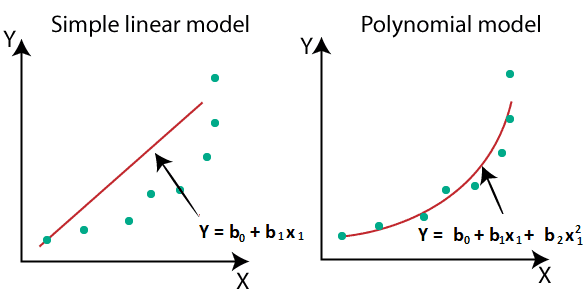
\includegraphics[width=0.7\textwidth]{img/regr_ex.png}
	\end{frame}
	
	
	\subsection{МНК}
	
	
	\begin{frame}
		\frametitle{Метод наименьших квадратов}
		Для решения такого рода задач применяется \textbf{метод наименьших квадратов} (МНК):
		
		$$
		Q(\theta, X) = \sum_{i=1}^{\ell} (a(x_i, \theta) - y_i)^{2} \to \min_{\theta}
		$$
		
		где $a(x, \theta)$ - некоторая \textbf{модель регрессии} (параметрическое семейство функций). $\theta = (\theta_1, ..., \theta_p)^{T}$
		
		\vspace{15pt}
		
		Результат оптимизации - набор конкретных значений параметров для выбранного семейства: 
		
		$$
		\theta^{*} = \arg \min_{\theta} Q(\theta, X)
		$$		
	\end{frame}

	\begin{frame}
		\frametitle{Решение оптимизационной задачи МНК}
		В случае дифференцируемости $a(x, \theta)$ по $\theta$, решение находится из системы из $p$ уравнений (необходимое условие минимума):
		
		$$
		\frac{\partial Q}{\partial \theta} = 2 \sum_{i=1}^{\ell} (a(x_i, \theta) - y_i) \frac{\partial a}{\partial \theta} = 0
		$$
		
		\vspace{15pt}
		
		Решая систему, получим обученную модель $a^{*}(x) := a(x, \theta^{*})$ описывающую зависимость $y$ от $x$ наилучшим образом (в среднеквадратичном смысле).		
	\end{frame}
	
	
	\begin{frame}
		\frametitle{Линейная регрессия}
		
		Частный случай, когда $a(x, \theta)$ линейна по своим параметрам - \textbf{линейная регрессия}
		
		$$
		a(x, \omega) = \omega_0 + \sum_{j=1}^{n} \omega_j x_j = 
		\omega_0 + \langle \omega, x\rangle 
		$$
		Определяется вектором коэффициентов $\omega = (\omega_1, ..., \omega_n) \in \mathbb{R}^{n}$ и свободным членом $\omega_0 \in \mathbb{R}$
		
		\vspace{5pt}
		
		Для упрощения формул добавим к признаковому описанию объектов признак равный единице 
		$$x := (1, x_1, ..., x_n), \
		 \omega := (\omega_0, \omega_1, ..., \omega_{n})$$
		 
		Тогда модель линейной регрессии:
		$$
		a(x) = \langle \omega, x \rangle
		$$
	\end{frame}	

	
	\begin{frame}
		\frametitle{Применение МНК к линейной модели}
		Удобно работать в матричной форме:
		
		$$ Q(\omega) = \|X\omega - y\|^{2} $$
		
		Необходимое условие минимума:
		
		$$ \frac{\partial Q}{\partial \theta} = 2X^{T} (X\omega - y) = 0$$
		
		$$ X^{T}X\omega = X^{T}y $$
		
		Аналитическое решение:
		$$ \omega^{*} = (X^{T}X)^{-1} X^{T} y $$
	\end{frame}


	\subsection{Мультиколлинеарность}
	
	
	\begin{frame}
		\frametitle{Проблема линейной зависимости признаков}
		Аналитическое МНК решение задачи линейной регрессии:
		
		$$ \omega^{*} = (X^{T}X)^{-1} X^{T} y $$
		
		\vspace{5pt}
		
		Если среди признаков (столбцов $X$) есть \textbf{линейно зависимые}, то определитель матрицы $X^{T}X$ равен нулю и её обращение $(X^{T}X)^{-1}$ невозможно! Следовательно, \textbf{решения нет}.
		
		\vspace{15pt}
		Если матрица имеет полный ранг, но столбцы \textbf{почти линейно зависимы} (сильная корреляция), то говорят что матрица плохо обусловлена.
	\end{frame}
	
	
	\begin{frame}
		\frametitle{Мультиколлинеарность}
		Почти линейную зависимость среди признаков называют \textbf{проблемой мультиколлинеарности}. Она ведет к:
		
		\vspace{5pt}
		
		\begin{itemize}
			\item \textbf{большой разброс} по абсолютной величине и знаку у коэффициентов $\omega^{*}$
			
			\item \textbf{неустойчивое обучение} - добавление или удаление нескольких объектов из $X$ влечет значительно разные оптимальные $\omega^{*}$
			
			\item \textbf{решение неустойчиво} - малое изменение входных данных влечет сильное изменение значения функции регрессии
		\end{itemize}
	\end{frame}
	
	\begin{frame}
		\frametitle{Методы борьбы с мультиколлинеарностью} 
		Для борьбы с мультиколлинеарностью можно:
		\begin{itemize}
			\item удалять скоррелированные столбы 
			\item вводить ограничения на параметры
			\item добавить штраф  в фунционале качества, зависящий от значений параметров (регуляризация)
		\end{itemize}
	\end{frame}
	
	
	\subsection{Регуляризация}
	
	
	\begin{frame}
		\frametitle{Квадратичная регуляризация - гребневая регрессия}
		\textbf{Метод гребневой регрессии} (Ridge regression) состоит в добавлении слагаемого, штрафующего за большие веса:
		
		$$Q_{\alpha}(\theta) = \|X\omega - y\|^{2} + \alpha \|\omega\|^{2}$$
		
		компоненту $\alpha \|\omega\|^{2}$ называют квадратичным регуляризатором, а параметр $\alpha$ - параметром регуляризации
		
		\vspace{15pt}
		
		В этом случае решение имеет вид:
		$$
		\omega_{\alpha}^{*} = (X^{T}X + \alpha E)^{-1} X^{T} y
		$$
		где $E$ - единичная матрица
	\end{frame}
	
	% подправить форматирование внутри скобки
	\begin{frame}
		\frametitle{Лассо - отбор признаков}
		Другая идея состоит в добавлении ограничения на сумму абсолютных значений весов. Называется \textbf{метод Лассо} (LASSO, Least Absolute Shrinkage and Selection Operator):
		
		\[
			\begin{cases}
				Q(\theta) = \|X\omega - y\|^{2} \rightarrow \min_{\omega}
				\\
				\sum_{j=0}^{n}|\omega_{j}| <= \beta
			\end{cases}
		\]
		
		параметр $\beta$ - селективность.
		
		
		Альтернативная формулировка метода:
		
		\[
		Q(\theta) = \|X\omega - y\|^{2} + \beta \|\omega\|_{1} \rightarrow \min_{\omega}
		\] 
		
		Особенность метода состоит в умении отбирать признаки. С уменьшением параметра $\beta$ становится "выгоднее" \textbf{занулять некоторые веса}.
	\end{frame}
	
	
	\begin{frame}
		\frametitle{Эффект от регуляризации}
		\begin{figure}[h]
			% for webp format:$ dwebp image.webp -o image.png
			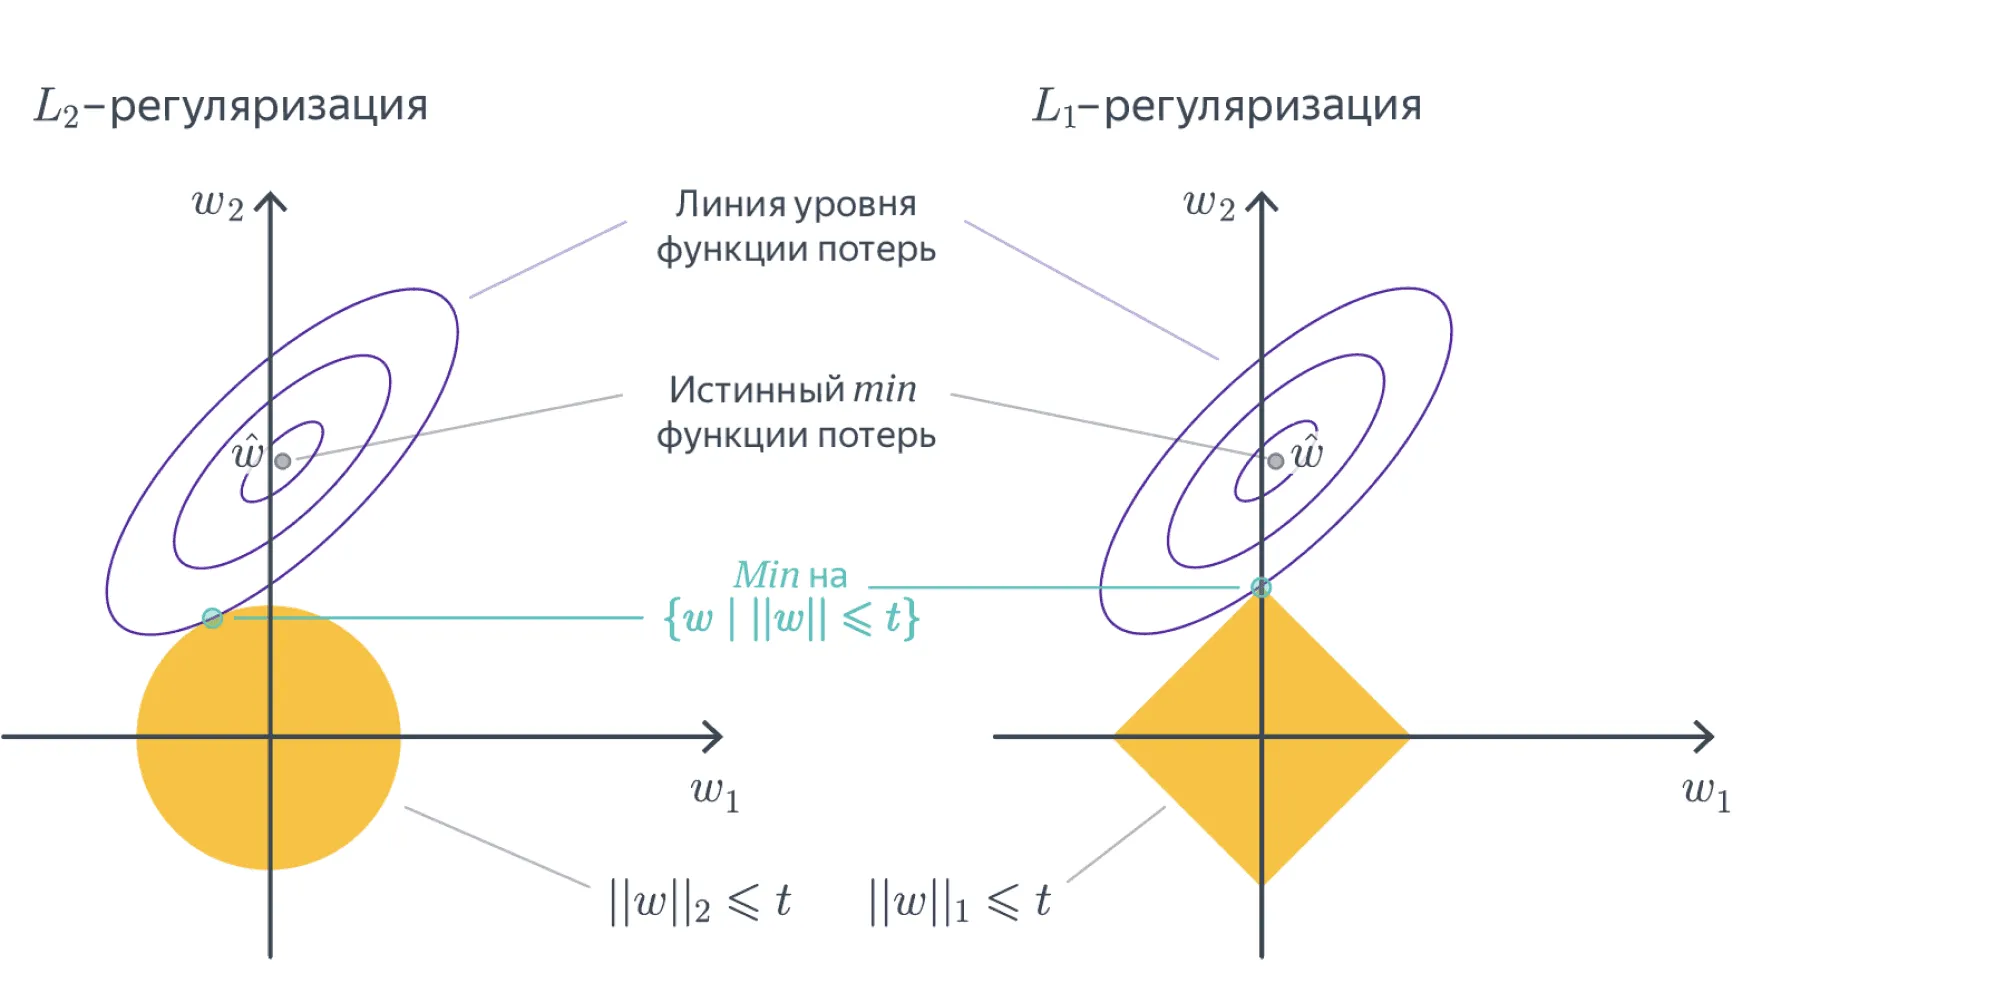
\includegraphics[width=\paperwidth, ]{img/l1_l2_regul.png}
		\end{figure}
	\end{frame}
	
	
	
	\section{Нелинейные обобщения}
	
	\subsection{Преобразования признаков}
	
	\begin{frame}
		\frametitle{Нелинейные преобразования признаков}
		Можно перейти от исходного признакового описания $x = (x_1, ..., x_n)$  к новым признакам $g(x) = (g_1(x), ..., g_m(x))$.
		
		\vspace{15pt}
		
		Например, вместо сложной модели (нелинейной по признакам)
		$a(x, \omega) = \omega_1 \ln(x_1) + \omega_2 \exp(x_2) + \omega_3 \frac{x_1}{x_2}$
		
		можно перейти к новому признаковому описанию $x^{'} = g(x)$, $g(x) = (\ln(x_1), \exp(x_2), \frac{x_1}{x_2})$.
		И тогда $a(x^{'}, \omega) = \omega_1 x_1^{'} + \omega_2 x_2^{'} + \omega_3 x_3^{'} = \langle w, x^{'} \rangle$ - линейная модель и по признакам, и по весам.
	\end{frame}
	
	\subsection{Нелинейная модель}
	
	\begin{frame}
		\frametitle{Нелинейная модель регрессии}
		Случай нелинейной модели $a(x, \omega)$ \textbf{по своим параметрам} $\omega$. Другими словами, модель нельзя представить скалярным произведением: $a(x, \omega) \ne \langle \omega, g(x) \rangle$ , где $g(x)$ - некоторое преобразование признаков, $g: \mathbb{R}^n \rightarrow \mathbb{R}^m$.
		
		\vspace{15pt}
		
		Примеры:
		\begin{itemize}
			\item $a(x, \omega) = x^{\omega}$ - нелинейная
			\item $a(x, \omega) = \sin(x_1 \omega_1) + \cos(x_2 \omega_2)$ - нелинейная
			\item $a(x, \omega) = \omega_1 \ln(x_1) + \omega_2 \exp(x_2)$ - \textbf{линейная}
		\end{itemize}
	\end{frame}
	
	
	\begin{frame}
		\frametitle{Обобщенные линейные модели}
		Огромный класс моделей образуют Обобщенные линейные модели (\textbf{GLM}, Generalized linear Models).
		
		\vspace{5pt}
		
		Идея в том, что модель регрессии линейна, но задана нелинейная функция связи $h(\cdot)$ между результатом модели и целевой переменной.
		
		\[
		a(x, \omega) = h(\langle \omega, x \rangle)
		\]
	\end{frame}
	
	\subsection{Другие функция потерь}
	
	\begin{frame}
		\frametitle{Другие функция потерь}
		Квадратичная функции потерь $\mathcal{L}(a, y) = (a(x) - y)^2$ соответствует методу наименьших квадратов. 
		
		\vspace{5pt}
		
		\begin{itemize}
			\item $\mathcal{L}(a, y) = |a(x) - y|$ - линейная
			\item $\mathcal{L}(a, y) = [a(x) \ne y]$ - 0-1 функция
			\item $\mathcal{L}(a, y) = \ln(1 + e^{- a(x) y})$ - логистическая
			\item $\mathcal{L}(a, y) = \max(0, 1 - a(x) y)$ - Hinge loss
		\end{itemize}
		
		\vspace{5pt}
		
		Необходимо подбирать функцию потерь которая лучшим образом описывающую бизнес требования задачи.
	\end{frame}
	
	
	\section{Градиентные методы оптимизации}
	
	
	\begin{frame}
		\frametitle{Решение задачи оптимизации}
		В случае не квадратичной функции потерь или нелинейной модели регрессии решение ищут численными методами.
		
		\[
		Q(a, X) = \sum_{i=1}^{\ell} \mathcal{L}(a(x_i, \omega), y_i) \rightarrow \min
		\]
		
		
		Вектор частных производных (градиент) по параметрам в общем виде :
	
		\[
		\frac{\partial Q}{\partial \omega_j} = \sum_{i=1}^{\ell} \frac{\partial \mathcal{L}}{\partial a} \cdot \frac{\partial a}{\partial \omega_j}
		\]
	\end{frame}
	
	
	\begin{frame}
		\frametitle{Численное решение}
		Наиболее простой и подходящий класс методов -- \textbf{градиентные методы оптимизации}.
		
		\vspace{5pt}
		
		\begin{wrapfigure}{r}{0.3\textwidth}
			\centering
			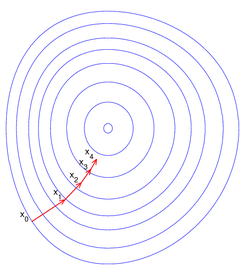
\includegraphics[width=0.35\textwidth]{img/grad.png}
		\end{wrapfigure}
		
		Общая схема:
		$$
		Q(\omega) = \sum_{i=1}^{\ell} \mathcal{L}_{i}(\omega) \to \min_{\omega}
		$$
		
		$$
		\omega^{(t + 1)} = \omega^{(t)} - \alpha \cdot \nabla_{\omega} Q(\omega^{(t)})
		$$
		где $\alpha \in \mathbb{R}$ - некоторый параметр (размер шага)
		
		\vspace{5pt}
		
		Градиент квадратичного функционала:
		
		$$
		\nabla_{\omega} Q = 2 X^{T}(X\omega - y)
		$$
	\end{frame}


	\begin{frame}
		\frametitle{Метод градиентного спуска}
		
		\begin{algorithm}[H]
			\caption{Метод градиентного спуска}
			\SetAlgoLined
			
			\KwIn{$\alpha$ - градиентный шаг (темп обучения)}
			\KwOut{$\omega^{*}$ - оптимум функцмонала $Q(\omega)$}
			\Begin{									
				Инициализировать $\omega^{(0)}$
				
				\While{не выполнен критерий остановки}
				{
					вычислить градиент в точке
					
					$\nabla Q(\omega)\at[\big]{\omega=\omega^{(t)}} = \left( \frac{\partial Q(\omega)}{\partial \omega} \right)_{i=1}^{n}$\;
					
					\vspace{5pt}
					
					сделать шаг в сторону антиградиента
					
					$\omega^{(t + 1)} = \omega^{(t)} - \alpha \cdot \nabla_{\omega} Q(\omega^{(t)})$\;
				}
			}
			
		\end{algorithm}
	\end{frame}
	
	
	\begin{frame}
		\frametitle{Идея ускорения алгоритма}
		Градиент $\nabla Q(\omega)$ представим в виде суммы градиентов:
		
		$$
		\nabla Q(\omega) = \frac{1}{\ell} \sum_{i=1}^{\ell} \nabla \mathcal{L}(\omega)
		$$
		
		Идея состоит в том, чтобы вычислять не точное значение градиента по всей выборке $X$, а оценить но некоторой подвыборке $X^{'} \subset X, |X^{'}| = k \ll \ell$ небольшого размера.
		
		$$\nabla Q(\omega) \approx \frac{1}{k} \sum_{i=1}^{k} Q(\omega)$$
		
		
	\end{frame}
	
	
	\begin{frame}
		\frametitle{Метод стохастического градиента}
		% 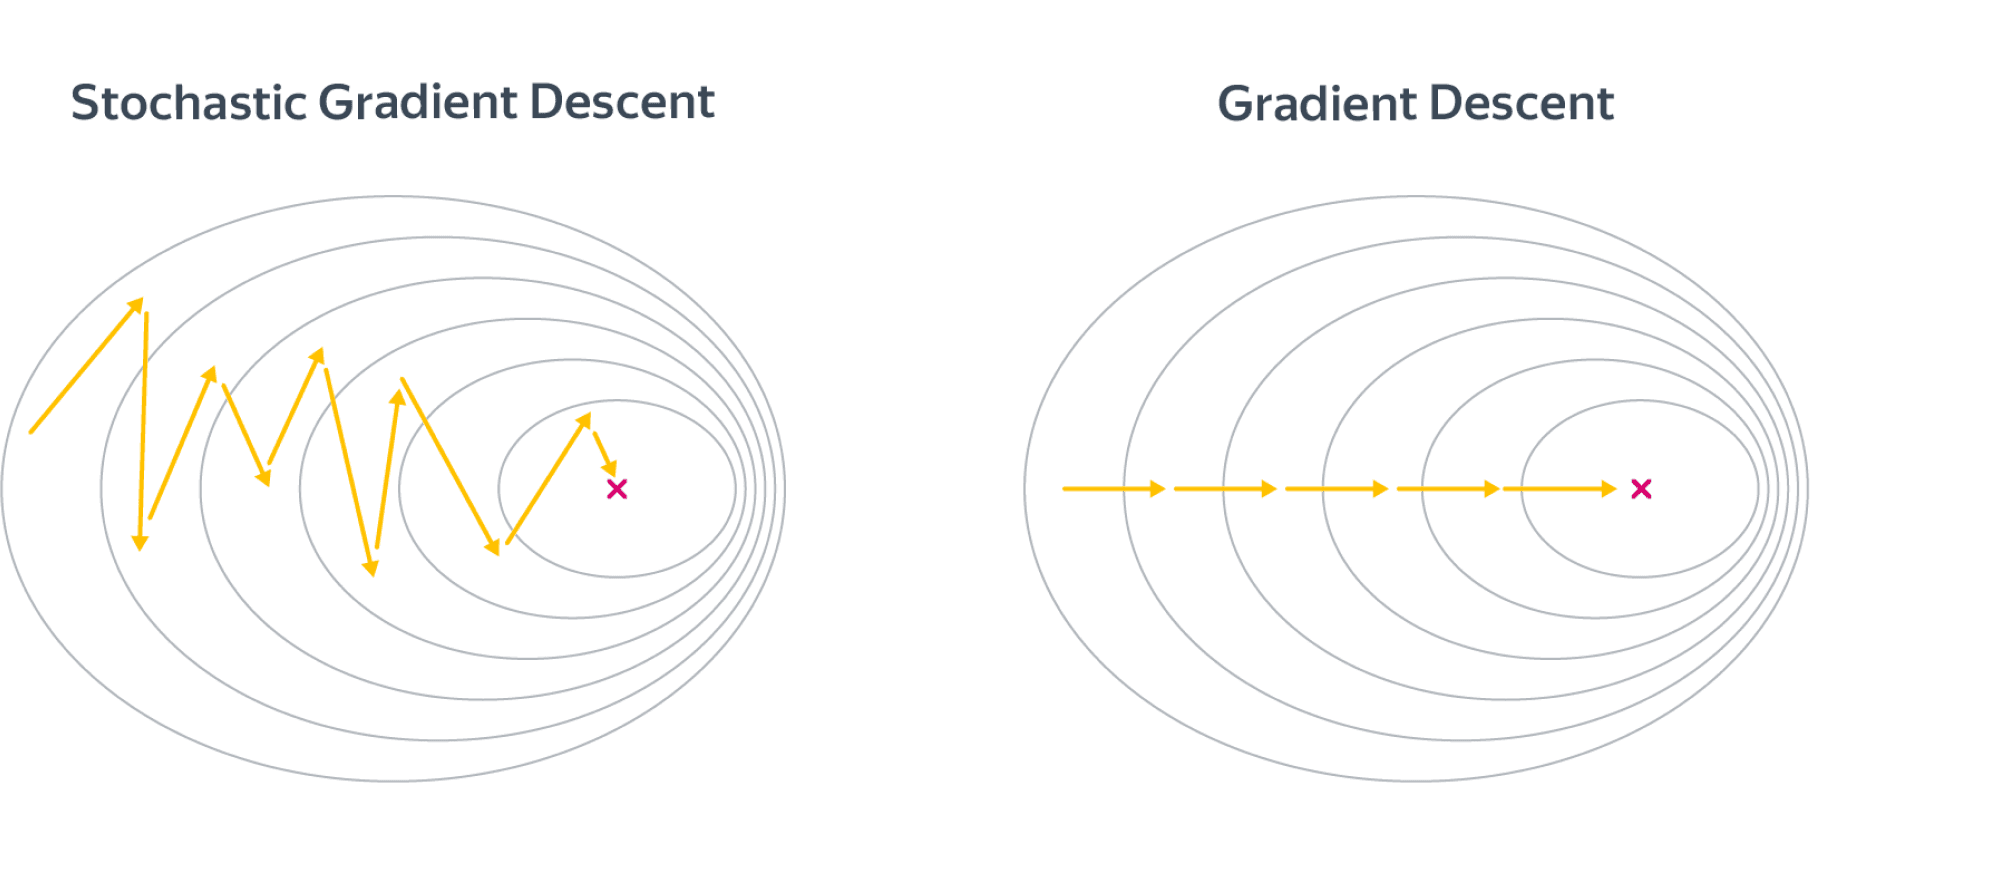
\includegraphics[width=\linewidth]{img/stoch_grad.png}
		
		\begin{algorithm}[H]
			\caption{Метод стохастического градиента}
			\SetAlgoLined
			
			\KwIn{$k$ - размер подвыборки, $\alpha$ - градиентный шаг}
			\KwOut{$\omega^{*}$ - оптимум функцмонала $Q(\omega)$}
			\Begin{
				Инициализировать $\omega^{(0)}$
				
				\While{не выполнен критерий остановки}
				{
					выбрать набор $X^{'}, |X^{'}| = k$
					
					\vspace{10pt}
					
					вычислить градиент в точке по подвыборке $X^{'}$
					
					$\nabla Q(\omega)\at[\big]{\omega=\omega^{(t)}} = \left( \frac{\partial Q(\omega)}{\partial \omega} \right)_{i=1}^{n}$\;
					
					\vspace{10pt}
					
					сделать шаг в сторону антиградиента
					
					$\omega^{(t + 1)} = \omega^{(t)} - \alpha \cdot \nabla_{\omega} Q(\omega^{(t)})$\;
				}
			}
		\end{algorithm}
	\end{frame}
	
	% оставлю на потом	
	\section{Вероятностная постановка задачи}
	


\end{document}